\documentclass{article}
\usepackage[utf8]{inputenc}

\title{Image Analysis and Computer Vision Homework}
\author{Parroni Federico}
\date{December 2018}

\usepackage{natbib}
\usepackage{graphicx}
\usepackage{mathtools}
\usepackage{hyperref}

\begin{document}
\maketitle

\vspace{1cm}
\tableofcontents

\newpage
\section{Image feature extraction and selection}

\subsection{Ellipsis detection}
The main ellipsis of interest in the image are the rims of the wheels. A built-in function of Matlab, \textit{regionprops}, has been used to find the ellipsis in the image.
The original image has been processed to help \textit{regionprops} to find correctly and precisely the wanted ellipsis.
At first, the original image is filtered to enhance the contrast. Then, for each wheel, an ad-hoc filtering process has been adopted:
\begin{itemize}
    \item Wheel 1: binarize the preprocessed image with a global threshold computed using Otsu's method, then apply the \textit{remove} filter (that set a pixel to 0 if its 4 neighbors are all 1, thus leaving only boundary pixels)
    \item Wheel 2: binarize again the original image, but with two different threshold values computed by changing the neighborhood size. At this point, we can sum the two thresholded images: in this way we can select white parts in both ones. Then, we apply a \textit{dilate} filter to reduce a bit the remaining black holes of the wheel rays
\end{itemize}
Now we can use \textit{regionprops} to get the parameters of some ellipsis in the image. From this set of elements, only the most significant are taken and we get rid off all the others, resulting in the following:
\begin{figure}[h!]
\centering
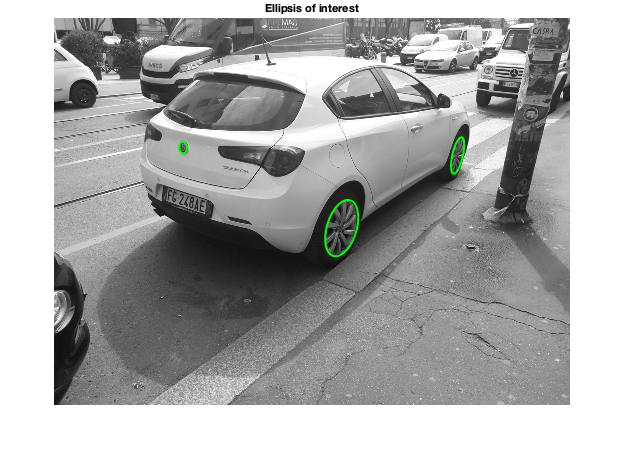
\includegraphics[scale=0.6]{images/homework_08.png}
\caption{Ellipsis}
\label{fig:ellipsis}
\end{figure}

\newpage
\subsection{Feature detection}
We can use the well-known Harris to extract features from the image. Corners are those pixels that have the response $E_{x,y}(r,c)$ to a sliding window $w$ (which captures each pixel neighbour) high:
$$ E_{x,y}(r,c) = \sum_{(u,v) \in U_{r,c}} w_{r,c}(u,v) [I(u,v) - I(u-x,v-y)]^2 $$
We can expand $ I(u-x,v-y)$ in Taylor series and considering only the first term we approximate:
$$ E_{x,y}(r,c) \approx \sum_{(u,v) \in U_{r,c}} w_{r,c}(u,v) [xI_x(u,v) + yI_y(u,v)]^2 $$
This can be rewritten in matrix form as:
$$ E_{x,y}(r,c) \approx (x,y) M_{r,c} \begin{pmatrix} x \\ y \end{pmatrix} $$
where: $ M_{r,c} = \begin{pmatrix}
I_x^2 \otimes w & I_x I_y \otimes w \\
I_x I_y \otimes w & I_y^2 \otimes w
\end{pmatrix} $. $I_x$ and $I_y$ are the image derivatives and are computed with a Gaussian filter in our case (with a certain standard deviation $\sigma$).
We can limit the analysis to only $M_{r,c}$, in particular looking to the eigenvalues we can establish if the pixel $(r,c)$ is a corner. In fact, for corners, both $\lambda_1$ and $\lambda_2$ are large. It is possibile to avoid computing the eigenvalues of $M_{r,c}$ evaluating another measure:
$$ CM = \frac{det(M_{r,c})}{Tr(M_{r,c}) + \epsilon} = \frac{(I_x^2 \otimes w)(I_y^2 \otimes w) - (I_x I_y \otimes w)^2}{(I_x^2 + I_y^2) \otimes w + \epsilon} $$
that is high if both eigenvalues are high.
\\
\\
I used the value $\sigma = 2.7$ for the standard deviation of the Gaussian filter (that controls the sensitivity of the filter) to avoid extracting too many and useless features.

\newpage
\section{Geometry}
\subsection{Diameter of wheel and wheel-to-wheel distance ratio}
We approach the computation of the ratio by finding a matrix $H_R$ such that, multiplied by an image point belonging to a plane, it gives back the rectified version of it. We can use $H_R$ to find the rectified wheels and then measure directly the diameter and the wheel-to-wheel distance. These are not the real measures (because we cannot find the original size with only this information), but since our goal is the ratio between two measures, this is good enough.
To compute $H_R$ we can resort to the \textit{conic dual to the circular points} and its image. This is:
$$ C_\infty^* = IJ^T + JI^T = \begin{pmatrix}
1 & 0 & 0 \\
0 & 1 & 0 \\
0 & 0 & 0
\end{pmatrix}
$$
and its image:
\begin{equation}
C_\infty'^* = I'J'^T + J'I'^T
\end{equation}
where $I = \bigl(\begin{smallmatrix}1 \\ i \\ 0 \end{smallmatrix} \bigr)$, $J = \bigl(\begin{smallmatrix}1 \\ -i \\ 0 \end{smallmatrix} \bigr)$ are the circular points (intersection between a circumference and the line at infinity) and $I'$, $J'$ their images.
Since a dual conic is transformed from a projective transformation H as:
$$ C'^* = H^* C^* H^T $$
we can exploit this relation to get $H_R$. In fact, in the case of $C_\infty^*$:
$$ C_\infty^* = H_R \: C_\infty'^* \: H_R^T = \begin{pmatrix}
1 & 0 & 0 \\
0 & 1 & 0 \\
0 & 0 & 0
\end{pmatrix}$$
If we explicit $C'^*$ from the above equation, we get:
\begin{equation}
C_\infty'^* = H_R^{-1} \: C_\infty^* \: H_R^{-T}
\end{equation}
So, if we know how the \textit{conic dual to the circular points} is mapped we can easily find $H_R$ using SVD (Singular Value Decomposition).
If fact, SVD decompose a matrix $A$ into 3 matrices:
$$ A = USV^T $$
In addition, if A is symmetric (and $C_\infty^*$ is), $U=V$. In our case:
$$ SVD(C_\infty'^*) = USU^T = H_R^{-1} \: C_\infty^* \: H_R^{-T} $$
resulting in $U=H_R^{-1}$.

\vspace{6mm}
The following steps have been followed:
\begin{enumerate}
    \item Find the images of the circular points starting from the two wheels (we know that they were circles and lie in a plane), by intersecting the 2 conics and the line at the infinity (findable thanks to the vanishing points)
    \item Compute $ C_\infty'^* $ as shown in equation 1
    \item Apply SVD to $ C_\infty'^* $ as shown in equation 2
    \item Get $ H_R = U^{-1} $
    \item Find 2 pairs of diametrically opposed points on the wheels
    \item Apply $ H_R $ to those points to get the rectificated points:
          $ \tilde{x_i} = H_R \: x'_i $
    \item Compute the ratio from this 4 points
\end{enumerate}

\begin{figure}[h!]
\centering
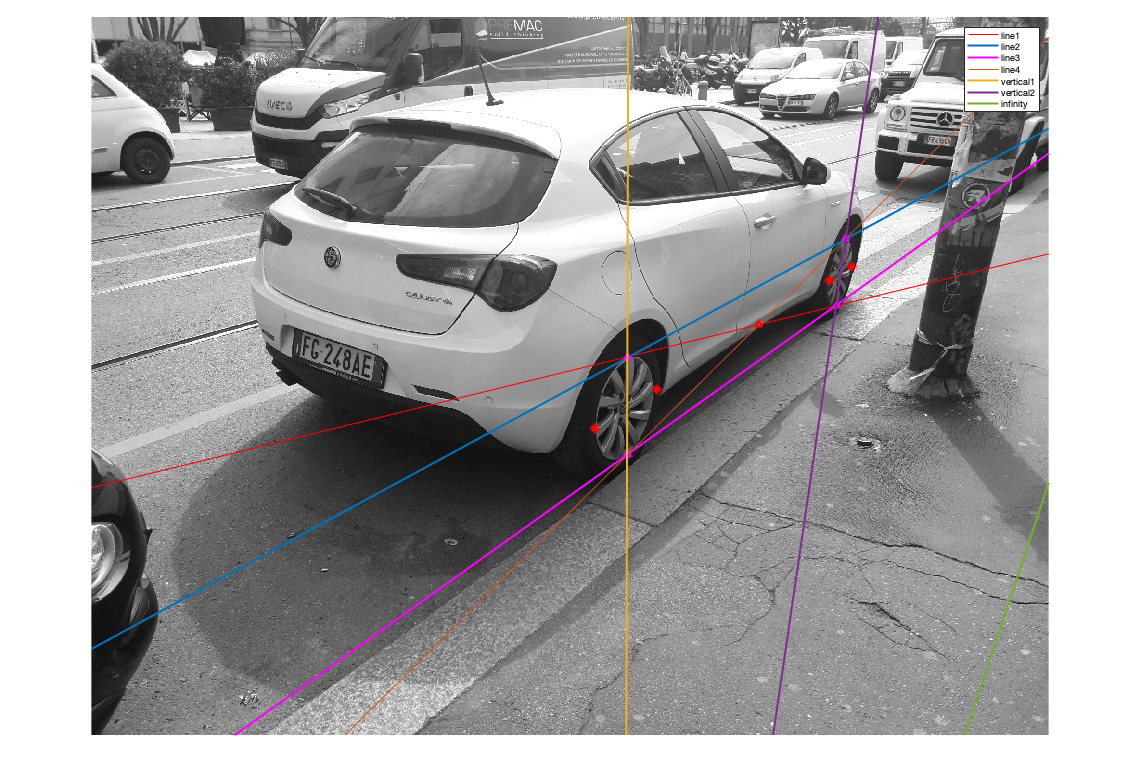
\includegraphics[scale=0.35]{images/homework_10.png}
\caption{Pairs of point to rectify and exploited lines}
\label{fig:rectification}
\end{figure}

The resulted ratio is: \textbf{0.1776}

\newpage
\subsection{Calibrate the camera determining the matrix K}
Under perspective projection, a scene point $X$ in space is projected to an image point $x$ via a projection matrix $P$ as:
\begin{equation}
\lambda x = PX = K \begin{pmatrix} R & t \end{pmatrix} \: X
\end{equation}
Calibration consists in finding the camera intrinsic parameters that compose the matrix K:
$$ K = \begin{pmatrix}
f_x & s & u_0 \\
0 & f_y & v_0 \\
0 & 0 & 1
\end{pmatrix}
$$
where $f_x$, $f_y$ are the camera’s focal length expressed in pixels, $(u0, v0)$ are the coordinates of the camera’s principal point expressed in pixels and $s$ is the skew factor (we can assume that $s = 0$).\\
This matrix can be found by considering the image of the \textit{absolute conic}. The absolute conic $\Omega_\infty$ is a conic on the plane at infinity, defined as:
$$ \begin{cases}
x^2 + y^2 + z^2 = 0 \\
w = 0
\end{cases}
$$
and so this coincides to:
$$
\Omega_\infty = \begin{pmatrix}
1 & 0 & 0 \\
0 & 1 & 0 \\
0 & 0 & 1
\end{pmatrix} = I
$$
Since a conic is transformed from a projective transformation H as:
$$ C' = H^{-T} C H^{-1} $$
applying the projection P to the \textit{image of the absolute conic} $\omega$, we obtain:
$$
\omega = P^{-T} \: I \: P^{-1} = (KR)^{-T} \: I \: (KR)^{-1} = (K^{-T}R) \: I \: (R^{-1}K^{-1}) = K^{-T}K^{-1}
$$
We notice that $\omega$ depends only on the camera calibration matrix K.
If we take the \textit{image of the dual absolute conic} $\omega^*$:
$$ \omega^* = \omega^{-1} = KK^T = \begin{pmatrix}
f_x^2+u_0^2 & u_0v_0 & u_0 \\
u_0v_0 & f_y^2+v_0^2 & v_0 \\
u_0 & v_0 & 1
\end{pmatrix}
$$
So, if we manage to find $\omega$, we have also found K. The \textit{image of the absolute conic} is a symmetric matrix and has 4 degrees of freedom, so we need to get 4 equations to fully determine it. For this scope, we can exploit the orthogonal vanishing points $v_x$, $v_y$, $v_z$ and one image of a circular point found before (that must belong to the conic), resulting in:
$$
\begin{cases}
v_x^T \: \omega \: v_y = \cos (90) = 0 \\
v_y^T \: \omega \: v_z = \cos (90) = 0 \\
v_z^T \: \omega \: v_x = \cos (90) = 0 \\
I'^T \: \omega \: I' = 0
\end{cases}
$$

\subsection{3D reconstruction of some pairs of symmetric features}
We initially need to fix a suitable reference frame for the world. From the information we have, we can get the rotation matrix R that relates the camera frame and the world frame:
$$ P = K \begin{pmatrix} R & t \end{pmatrix} $$
$R$ can be computed considering how a direction is projected to a vanishing point in the image. If we take equation 3 and we consider, for example, $X = V_x = \bigl(\begin{smallmatrix} 1 \\ 0 \\ 0 \\ 0 \end{smallmatrix} \bigr)$:
$$ \lambda v_x = K \begin{pmatrix} R & t \end{pmatrix} \: \begin{pmatrix} 1 \\ 0 \\ 0 \\ 0 \end{pmatrix} =
K \begin{pmatrix} r_1 & r_2 & r_3 & t \end{pmatrix} \: \begin{pmatrix} 1 \\ 0 \\ 0 \\ 0 \end{pmatrix} = 
K \: r_1
$$
where $r_i$ is the $i^{th}$ column of the matrix $R$.
Since the location of the vanishing point $v_x$ can be easily found in the image, we can get $r_1$:
$$ r_1 = K^{-1} \: v_x $$
Using the knowledge about the mapping between directions and vanishing points, we can obtain all the 3 columns of the $R$ (the last column can be obtained as cross product between the other two, since the columns of a rotation matrix have to be orthogonal each other). The vanishing point in the image are taken from orthogonal planes of the car, i.e. the right plane containing the wheels and the back plane containing the plate.
\\
\\
Let's initially set $t=0$, so this temporary world frame $W^0$ and the camera frame have the same orign but different rotation. In this setting, we know that the plate of the car lies on a certain vertical plane $\Pi_p$ in the form $z=k$. Since we have a degree of freedom due to the fact that we cannot know the exact measure of any distance (from a single image), let's arbitrarily fix this plane to $z=1$.
\\
Now, let's consider the viewing rays of two symmetric image points $d_1$, $d_2$ in the car plate plane (I decided to take two symmetric points located at the right and left border of the plate). Each of them is in the form:
$$ ray = (KR)^{-1}d_i = M^{-1}d_i $$
We know that these rays pass through the viewpoint $O$ of the camera:
$$ O = RNS(P) $$
The equation of the ray with direction $(l, m, n)$ passing through $O = (x_0, y_0, z_0)$ is:
$$ \frac{x-x_0}{l} = \frac{y-y_0}{m} = \frac{z-z_0}{n} $$

We want to fix the world frame $W^1$ such that it lies in the car symmetry plane $\Pi_{sym}$ (we know that this plane is vertical and also orthogonal to $\Pi_p$, so it has equation $x=k$). So, we can intersect two viewing rays of a pair of symmetric features with $\Pi_{p}$ and then take the midpoint as the origin $O_{W^1}$ of the new frame:
$$ O_{W^1} = ( x_s = \frac{x_1+x_2}{2}, \: \frac{y_1+y_2}{2}, \: \frac{z_1+z_2}{2}=1 ) $$
The symmetry plane $\Pi_{sym}$ will be:
$$ x=x_s $$

\begin{figure}[h!]
\centering
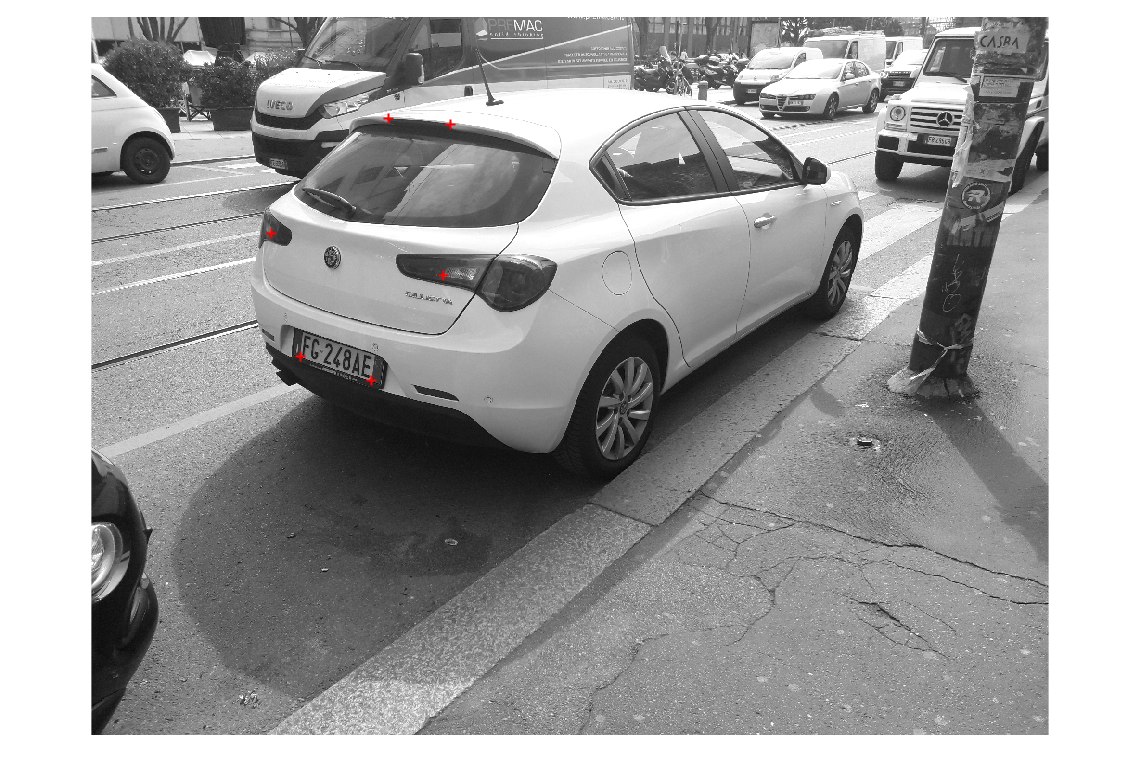
\includegraphics[scale=0.35]{images/homework_14.png}
\caption{Pairs of symmetric points}
\label{fig:symmetricfeatures}
\end{figure}

\newpage
Now that we have found $\Pi_{sym}$, all other symmetric points that lies on a different plane from $z=1$ can be found by imposing the following system of equations:
$$ \begin{cases}
\frac{x_1-x_0}{l_1} = \frac{y_1-y_0}{m_1} = \frac{z_1-z_0}{n_1} & \quad P_1 \text{ satisfies equation of ray 1} \\
\frac{x_2-x_0}{l_2} = \frac{y_2-y_0}{m_2} = \frac{z_2-z_0}{n_2} & \quad P_2 \text{ satisfies equation of ray 2} \\
z_1 = z_2 & \quad P_1 \text{ and } P_1 \text{ are in the same vertical plane} \\
\frac{x_1 + x_2}{2} = x_s & \quad P_1 \text{ and } P_1 \text{ are symmetric w.r.t } \Pi_{sym} \\
\end{cases} $$
where $d_1 = (l_1, m_1, n_1)$ and $d_2 = (l_2, m_2, n_2)$ are the viewing rays
passing though the two unknown intersection points $P_1 = (x_1, y_1, z_1)$ and $P_2 = (x_2, y_2, z_2)$ respectively.
\\
We can repeat this process multiple times for other pairs of symmetric points visible in the image. (\ref{fig:3dreconstructionW0})
\begin{figure}[hbt!]
\centering
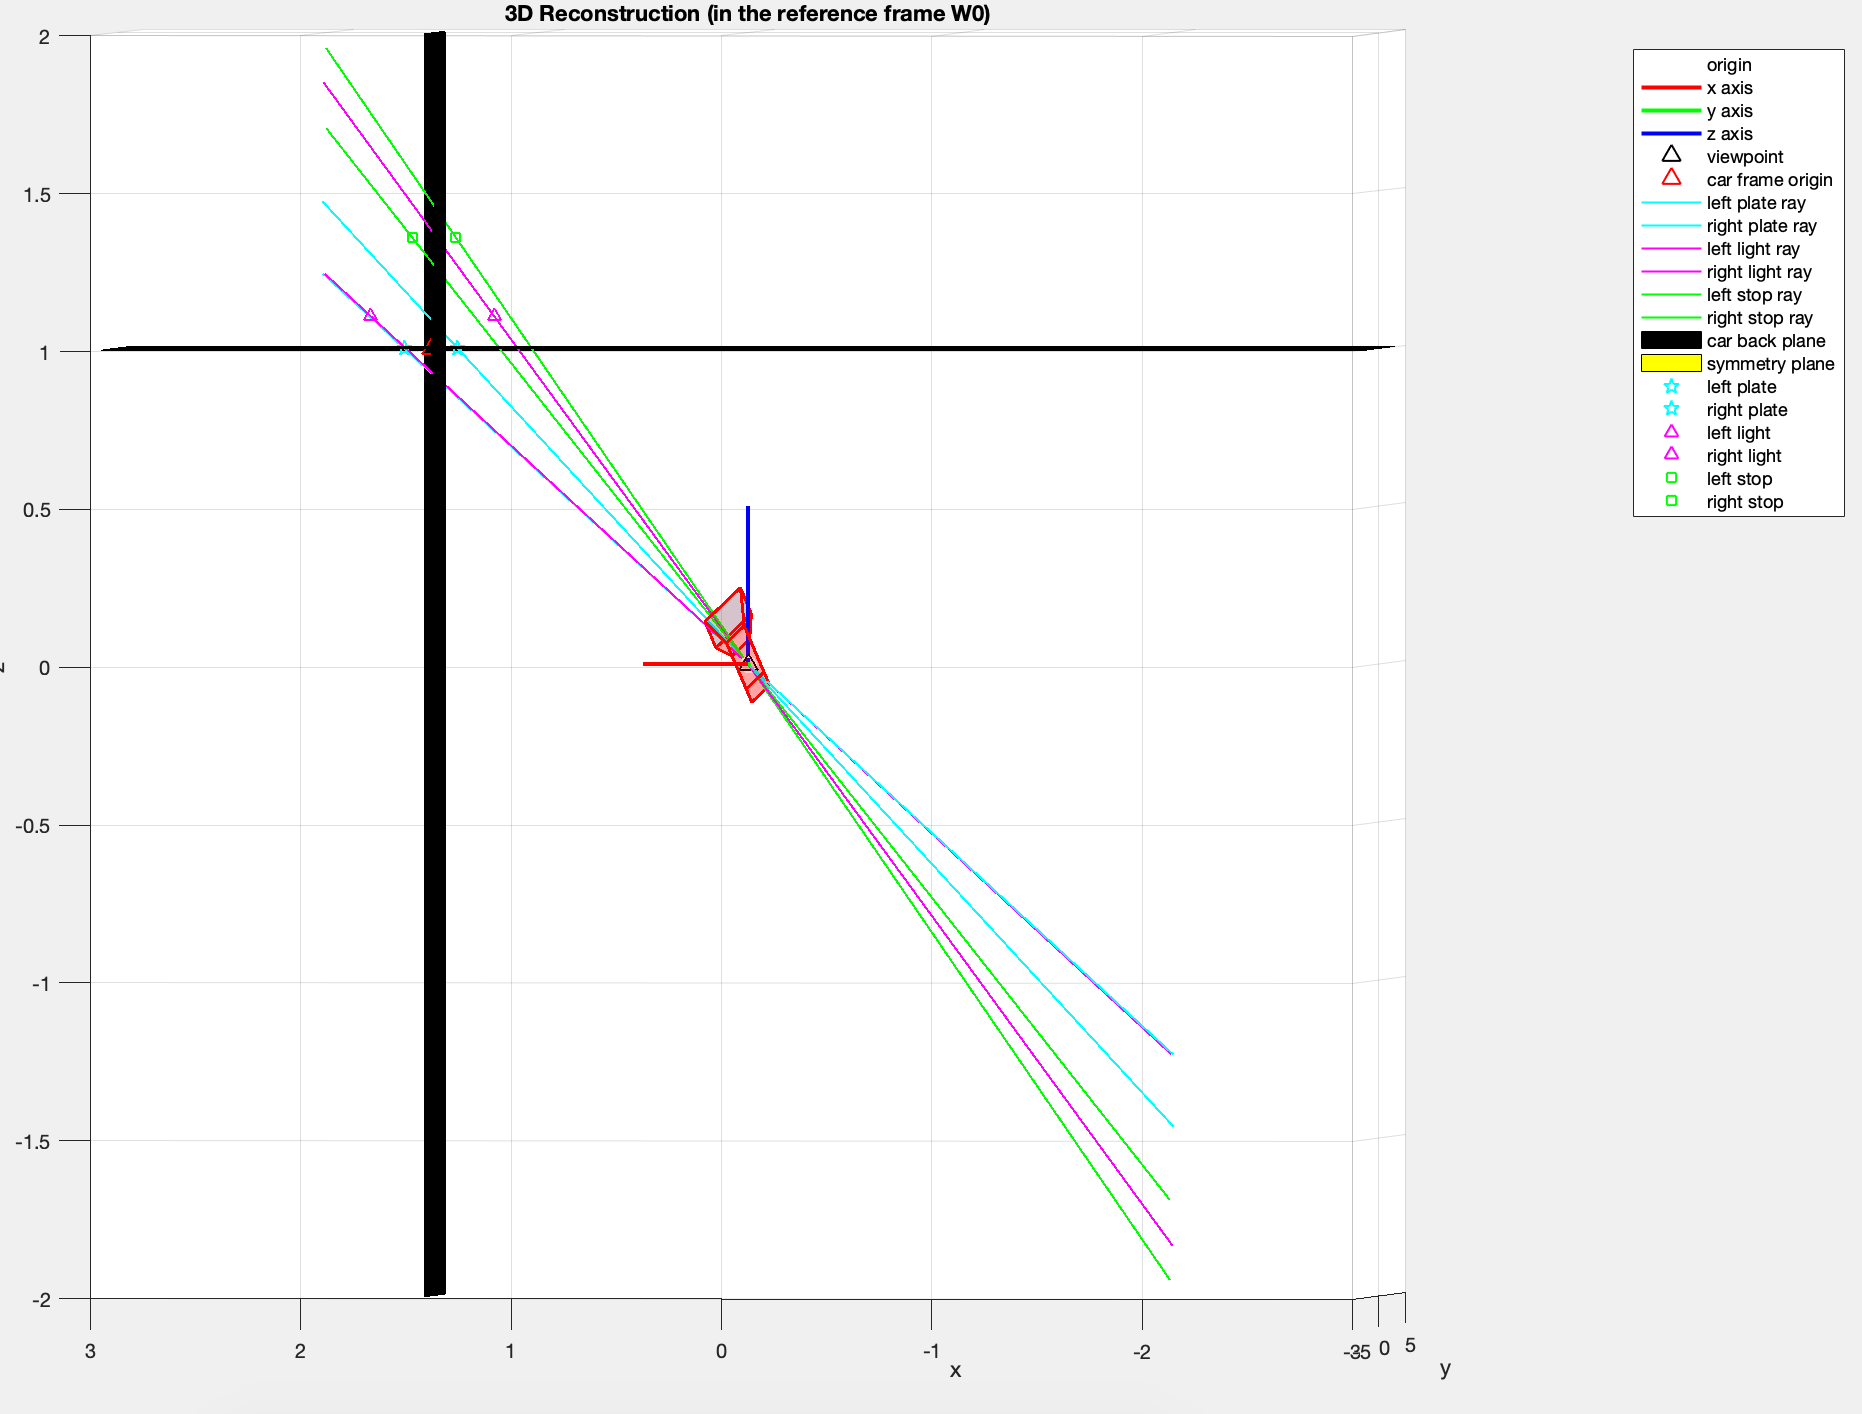
\includegraphics[scale=0.4]{images/3DreconstructionW0.png}
\caption{Symmetric points in the reference frame $W^0$}
\label{fig:3dreconstructionW0}
\end{figure}
\\

These points are expressed in the reference frame $W^0$. To change reference frame to $W^1$, we can compute the matrix that allows to pass from $W^0$ to $W^1$:
\begin{equation}
T_{W_0 \rightarrow W_1} = \begin{pmatrix} \multicolumn{3}{c}{I_{3 \times 3}} & -O_{W^1} \\
0 & 0 & 0 & 1
\end{pmatrix}
\end{equation}
where $O_{W^1}$ is the origin of $W^1$ expressed in the coordinates of the frame $W^0$ (notice that the two reference frames have the same orientation by construction). (\ref{fig:3dreconstructionW1})
\begin{figure}[hbt!]
\centering
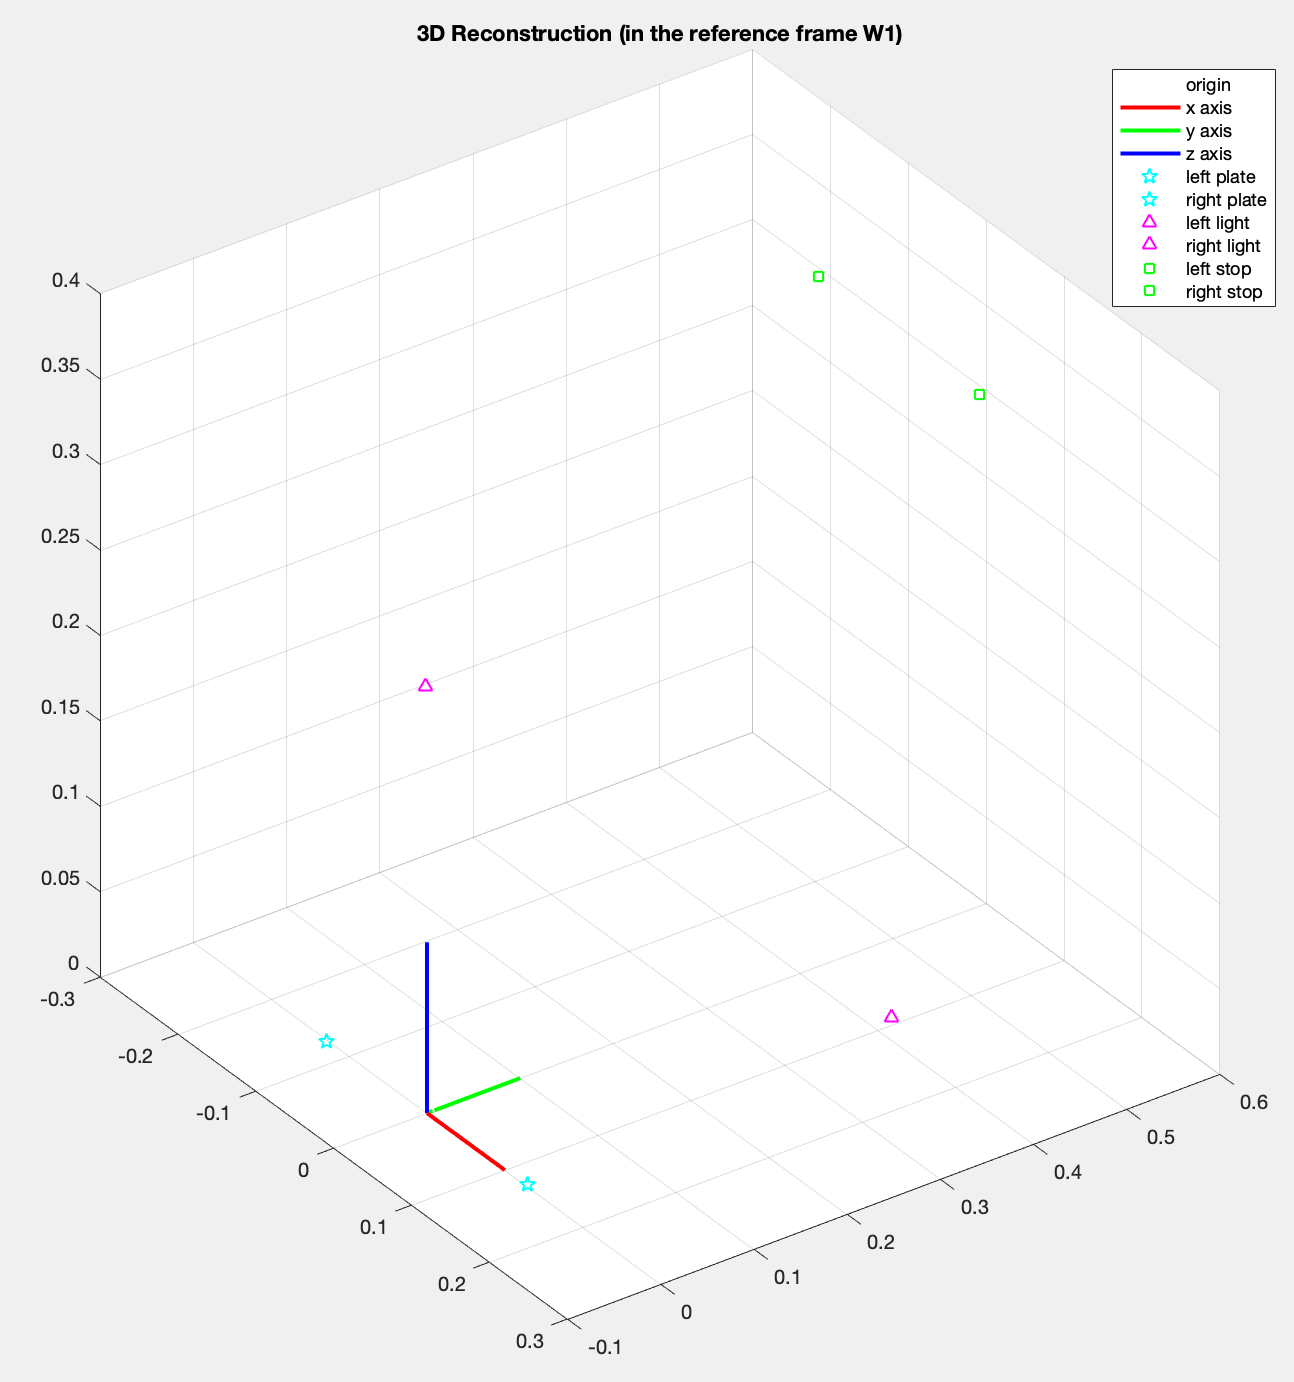
\includegraphics[scale=0.45]{images/3DreconstructionW1.png}
\caption{Symmetric points in the reference frame $W^1$}
\label{fig:3dreconstructionW1}
\end{figure}

\newpage
\subsection{Localize the camera relative to the car reference}
In the last section, when we have fixed the origin of the world frame $W^1$, we have also established the translation between the temporary reference frame $W_0$ and the world frame. In fact, at first, the two frames were coincident, so $t=(0, 0, 0)$. Then, the world frame $W_1$ has been set to a specific point $O_{W^1}=(x_0, y_0, z_0)$. Since the two frame have the same orientation, this corresponds to a pure translation by a vector:
$$ t_{W_1 \rightarrow W_0} = -t_{W_0 \rightarrow W_1} = (-x_0, \: -y_0, \: -z_0) $$
Thus the position of the camera can be obtained by translating the origin of $W_0$ (that was coincident to the camera location) by the above vector:
$$ P_{cam}^{W_1} = P_{cam}^{W_0} + t_{W_1 \rightarrow W_0} = \begin{pmatrix}
0 \\ 0 \\ 0
\end{pmatrix} + (-x_0, \: -y_0, \: -z_0) = (-x_0, \: -y_0, \: -z_0) $$
\\
We can get to the same result by applying the matrix $T_{W_0 \rightarrow W_1}$ (4) to the origin of the frame $W_0$:
$$ P_{cam} = T_{W_0 \rightarrow W_1} * P_{cam}^{W_0} = T_{W_0 \rightarrow W_1} * \begin{pmatrix}
0 \\ 0 \\ 0 \\ 1
\end{pmatrix} = -O_{W^1} =  (-x_0, \: -y_0, \: -z_0) $$
The numerical result obtained is:
$$ P_{cam} = \begin{pmatrix}
-1.4875 \\ 0.6788 \\ -1
\end{pmatrix} $$

\begin{figure}[hbt!]
\centering
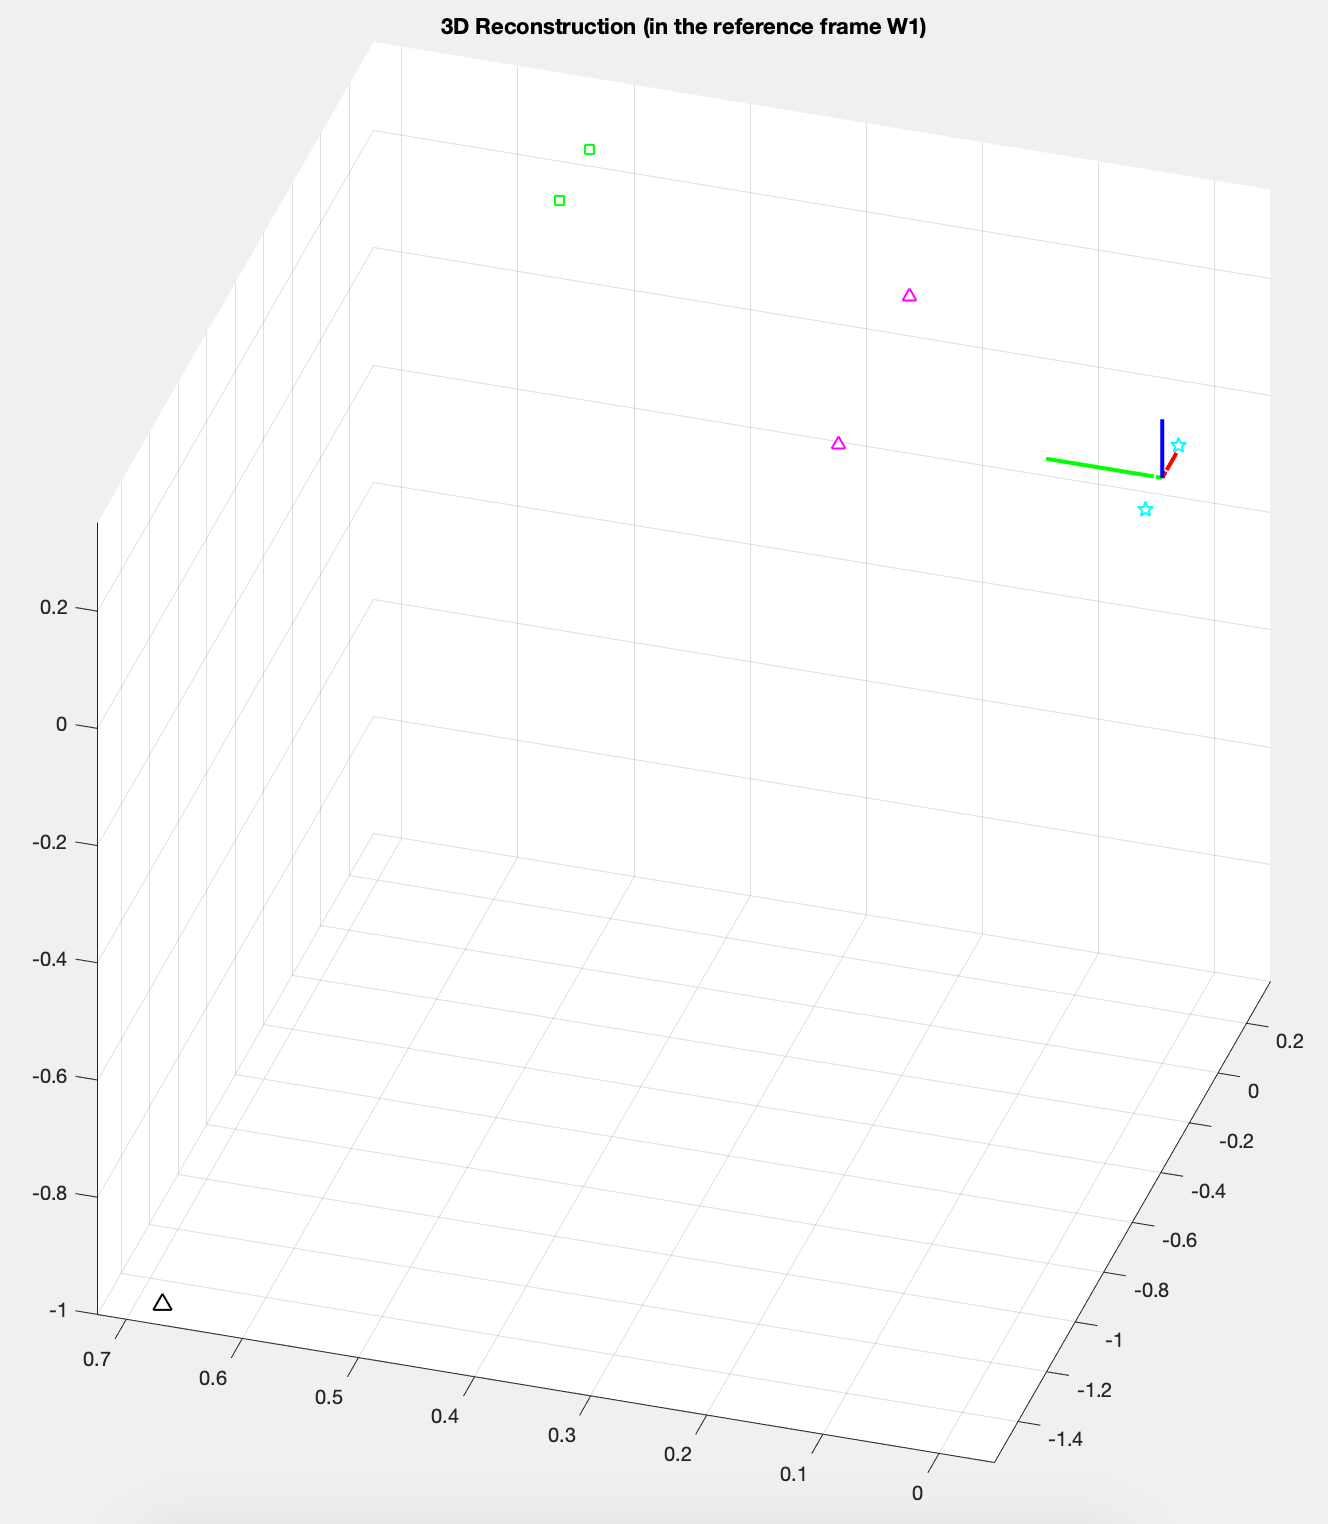
\includegraphics[scale=0.45]{images/cameralocation.png}
\caption{Camera location}
\label{fig:cameralocation}
\end{figure}

\newpage
\subsection{Comparison with the test image}
The camera calibration matrix obtained from the first image is the following:
$$ K = \begin{pmatrix}
0.7820 & 0 & 0.5781 \\
0 & 0.7778 & 0.4762 \\
0 & 0 & 1
\end{pmatrix} $$
I calibrated the camera also using the second image as countercheck (see homework\_test.html for further details). The result obtained is the following matrix:
$$ K = \begin{pmatrix}
0.9191 & 0 & 0.4921 \\
0 & 0.886 & 0.1861 \\
0 & 0 & 1
\end{pmatrix} $$

\newpage
\section{Analysis of the experimental results}

\subsection{Wheel diameter and wheel-to-wheel distance ratio}
The ratio we found in the first image is 0.1776.
\\
Looking for the car producer technical sheet, we know that the real wheel-to-wheel distance is 2.634m (and it is a standard for all cars of that model). If we suppose that the car wheel diameter is 18 inches (0.4572m), we get a ratio of: $\frac{0.4572}{2.634} = 0.174$, pretty close to the experimental result.
\\
\\
The ratio we found in the second image is 0.1904.

\subsection{3D reconstruction}
We found that the two symmetric points of the car plate are in the following locations in the frame $W_1$:
$$ p_1 = \begin{pmatrix}
0.1553 \\ 0 \\ 0
\end{pmatrix}
$$
$$ p_2 = \begin{pmatrix}
-0.1553 \\ 0 \\ 0
\end{pmatrix}
$$
while the camera is in:
$$ p_{cam} = \begin{pmatrix}
-1.4875 \\ 0.6788 \\ -1
\end{pmatrix}
$$
The car plate width is: $0.1553 + 0.1553 = 0.3106$.\\
If we can know the real car plate width, we can also rebuild the entire scene in the real scale.
The italian car plate has a standard size of 0.53m. Thus the scale factor we have is about:
$$ f = \frac{0.53}{0.31} = 1.71 $$
If we don't consider the y coordinate, the camera is $\sqrt{(-1.4875)^2 + (-1)^2} = 1.7924$m far from the center of the car plate (located in the origin of $W_1$).
So, the distance of the camera from the car plate center is:\\
$$ f*1.7924 = 1.71*1.7924\textit{m} = 3.07 \textit{m}$$


\newpage
\section{References}
All files of this homework can be found in my Github repo: \\
\\
\url{https://github.com/keyblade95/IACVhomework.git}

\newpage
\bibliographystyle{plain}
\bibliography{references}

\end{document}